\chapter{Risultati dei Algoritmi di machine learning}
\label{cap:RisML}
%**************************************************************
\intro{Questo capitolo illustrerà i risultati ottenuti dai algoritmi K-Nearest-Neighbors (K-NN),  Support Vector Machine (SVM), Decision Tree, Random Forest e infine AdaBoost.  
}

\section{Premesse}
Si sottolinea che, purtroppo, i metodi di \emph{machine learning} non consentono un'analisi interpretativa dei dati come i metodi di \emph{data mining}. Per questo verranno presentati solo i risultati delle predizioni con le relative metriche.\\
Durante la fase di \emph{preprocessing}, i dati sono stati standardizzati attraverso la funzione \textsf{StandardScaler()} del linguaggio Python, ovvero tutti i dati per ogni \emph{feature} sono stati centrati per ottenere media 0 e varianza 1. Questa operazione è stata eseguita per poter rendere le \emph{features} comparabili tra loro. Come già verificato nel Capitolo \ref{cap:Analisi} non ci sono valori mancanti. Durante la fase di \emph{feature selection} si utilizzano le stesse \emph{features} del modello Bradley-Terry escludendo ancora il numero di gol fatti dalla squadra in casa e dagli ospiti. Questo perché, durante una prima fase iniziale di verifica degli algoritmi, i metodi Decision Tree e Random Forest, grazie a queste \emph{feature}, ottenevano un’accuratezza pari a 1. Infatti, sapere il numero di gol segnati in una partita indica implicitamente l'esito della partita stessa. Quindi per non rendere inutili le altre \emph{feature}, il numero di gol segnati dalla squadra in casa e dagli ospiti non sono stati presi in considerazione. Ciononostante, si sottolinea la bontà dei due algoritmi che sono riusciti a trovare la correlazione precedentemente illustrata. Quindi le 26 \emph{features} scelte diventeranno 52, una metà delle quali si riferiscono alla squadra in casa, in cui ogni features viene indicata con il prefisso \textsf{Home\_}, mentre l'altra metà si riferisco alla squadra ospite, in cui ogni features viene indicata con il prefisso \textsf{Away\_}. L'attività di predizione verrà condotta suddividendo il \emph{dataset} in un insieme di training (80\%) e uno di test (20\%). La funzione utilizzata per rendere utilizzabile il \emph{dataset} è indicata nella Sezione \ref{code:a9}.

\section{Ulteriori metriche}
La capacità predittiva di un modello sarà valutata con le metriche illustrate nel Capitolo \ref{cap:risultatiDM} e con la seguente metrica.
\begin{itemize}
	
	\item \textsf{Area Under the Curve}. La Area Under the Curve (AUC) rappresenta l'area al di sotto della curva ROC, che è una rappresentazione grafica del rapporto tra specificità e sensibilità.
	L'AUC è una metrica che va da 0 a 1, dove un valore più alto indica una migliore prestazione di classificazione. L'AUC permette di confrontare le performance di classificatori diversi, poiché è indipendente dalla soglia di classificazione e fornisce un riassunto delle prestazioni del classificatore.
\end{itemize}

\section{K-Nearest-Neighbors}
L'algoritmo K-Nearest-Neighbors è risultato essere semplice da applicare, ottenendo complessivamente discreti risultati in fase di predizione. Per scegliere i valori migliori per gli iperparametri si è applicato la K-Fold Cross Validation con \emph{k = 10}.\\
Gli iperparametri valutati sono stati i seguenti:
\begin{itemize}
	\item \textsf{n\_neighbors}. Indica il numero massimo di vicini da considerare. Si sono verificati i valori da 3 fino a 163 vicini con un aumento unitario di 1.
	\item \textsf{p} indica il parametro potenza della distanza di Minkowski. Si sono verificati i valori \emph{p=1} (Manhattan distance) e \emph{p=2} (Euclidean distance).
\end{itemize}

Nella Figura \ref{fig:knnCV} viene mostrato l'andamento della Cross Validation per ogni valore degli iperparametri.
\begin{figure}[h]
	\begin{center}
		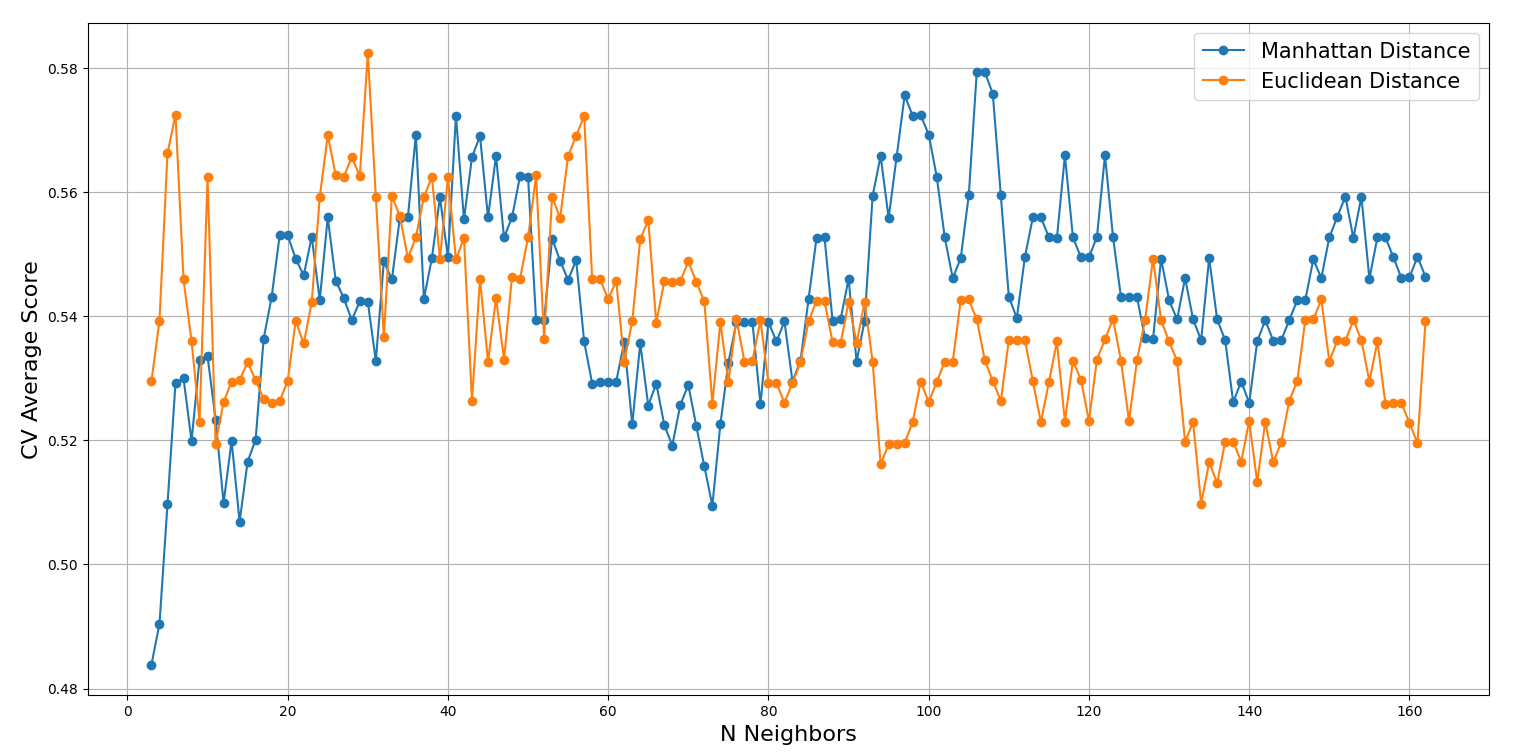
\includegraphics[scale=0.35]{knnCV.png}
		\caption{Grafico dell'andamento della media dell'accuratezza per ogni valore dell'iperparametro \textsf{n\_neighbors} e per ogni tipo di metrica di distanza utilizzata durante l'applicazione della Cross Validation con 10 fold per il modello K-Nearest-Neighbors. Ogni punto è un classificatore con un certo numero di vicini. La linea blu indica l'andamento con la distanza di Manhattan, mentre la linea arancione l'andamento con la distanza euclidea.
		} 
		\label{fig:knnCV}
	\end{center}
\end{figure}

Quello che si può notare dalla figura è che inizialmente, con pochi vicini, la distanza euclidea risulta essere migliore nella fase di training nel \emph{validation} \emph{set}, ma, con l'aumentare del numero dei vicini, la distanza di Manhattan ottiene risultati migliori. \\
Secondo la Cross Validation i valori migliori sono stati: il valore 30 come numero di vicini e la distanza euclidea come metrica della distanza da utilizzare. L'accuratezza ottenuta dal modello migliore nel \emph{validation} \emph{set} è stata di 0.582.\\
Nella fase di predizione si sono ottenute le predizioni mostrate nella Figura \ref{fig:knnpre} con le relative metriche presentate nella Figura \ref{fig:knnmetrics}.

\begin{figure}[h]
	\begin{center}
		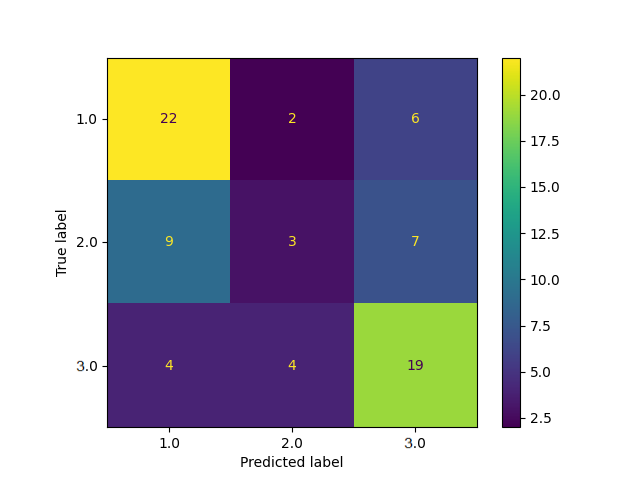
\includegraphics[scale=0.60]{tabknn.png}
		\caption{Tabella di confusione del modello K-Nearest-Neighbors con\textsf{ n\_neighbors} = 30 e \textsf{p} = 2. La classe 0.0 indica la vittoria della squadra in casa, la classe 1.0 indica il pareggio tra le due squadre, la classe 2.0 indica la vittoria della squadra ospite.
		} 
		\label{fig:knnpre}
	\end{center}
\end{figure}

\begin{figure}[h]
	\begin{center}
		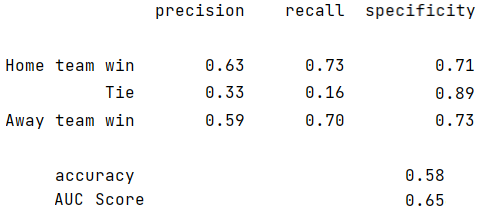
\includegraphics[scale=0.60]{metricknn.png}
		\caption{Grafico delle misurazione durante la fase di predizione del modello K-Nearest-Neighbors con\textsf{ n\_neighbors} = 30 e \textsf{p} = 2.
		} 
		\label{fig:knnmetrics}
	\end{center}
\end{figure}
I risultati ottenuti sono discreti. Infatti, l'accuratezza del modello nella fase di predizione è di 0.58. Il modello ha molta difficoltà a riconoscere quando un’osservazione è di classe pareggio dato che la sensibilità è pari 0.16 ovvero, delle 19 osservazioni effettivamente di classe pareggio solo tre vengono riconosciute come tali. Purtroppo, quando le osservazioni vengono etichettate con il pareggio, molto spesso viene commesso un errore di classificazione, dato che la precisione è pari a 0.33 ovvero, solo tre osservazioni su nove %che sono state etichettate con la classe pareggio
sono effettivamente di classe pareggio. Il modello, commettendo relativamente un numero di errori basso, ha una specificità pari a 0.89. Risultati discreti si ottengono per la classe vittoria della squadra in casa e vittoria della squadra ospite. La precisione del modello nella classe vittoria della squadra in casa è pari a 0.63. Infatti, 13 osservazioni vengono etichettate erroneamente con la classe vittoria della squadra in casa. La specificità risulta pari a 0.71 mentre la sensibilità della classe vittoria della squadra in casa è pari a 0.73 ovvero, otto osservazioni su trenta non sono state identificate di classe vittoria della squadra in casa. La precisione della classe vittoria della squadra ospite è pari 0.59 poiché sono stati commessi tanti errori di classificazione. Infatti, 13 osservazioni su 32 sono state etichettate erroneamente con la classe vittoria della squadra ospite. Invece la sensibilità registrata per la classe vittoria della squadra ospite è pari a 0.70 dato che solo otto osservazioni non sono state riconosciute appartenenti alla classe vittoria della squadra ospite. Analogamente, anche la specificità della classe vittoria della squadra ospite e buona dato che è pari a 0.73. Perciò, il modello riesce ad individuare quasi tutte le osservazioni di classe vittoria della squadra in casa o di classe vittoria della squadra ospite, anche se per entrambe le due classi ha una discreta precisione a causa di molte istanze di classe pareggio etichettate erroneamente.\\
Risulta non essere particolarmente adatto l'algoritmo K-Nearest-Neighbors per quest'analisi, a causa della grande diversità tra partita e partita. Ciononostante, si ottengono discreti risultati tenendo conto del fatto delle poche osservazioni messe a disposizione.
\section{Support Vector Machine}
L'algoritmo Support Vector Machine ha ottenuto dei buoni risultati durante la fase di predizione. Analogamente all'algoritmo K-Nearest-Neighbors, si è applicata la K-Fold Cross Validation con \emph{k = 10} per individuare i valori migliori per gli iperparametri.\\
Gli iperparametri valutati sono stati i seguenti:
\begin{itemize}
	\item \textsf{C}. Indica la forza applicata della penalità L2. Si sono verificati valori che vanno da 0.1 a 1.5 con un aumento unitario di 0.1.
	\item \textsf{kernel}. Indica quale funzione di kernel utilizzare. Si sono verificati i valori kernel = linear ovvero il linear kernel, kernel = rbf ovvero Gaussian Radial Basis kernel (RBF) e kernel = poly ovvero il polynomial kernel.
\end{itemize}

Nella Figura \ref{fig:svcCV} viene mostrato l'andamento della Cross Validation per ogni valore degli iperparametri.
\begin{figure}[]
	\begin{center}
		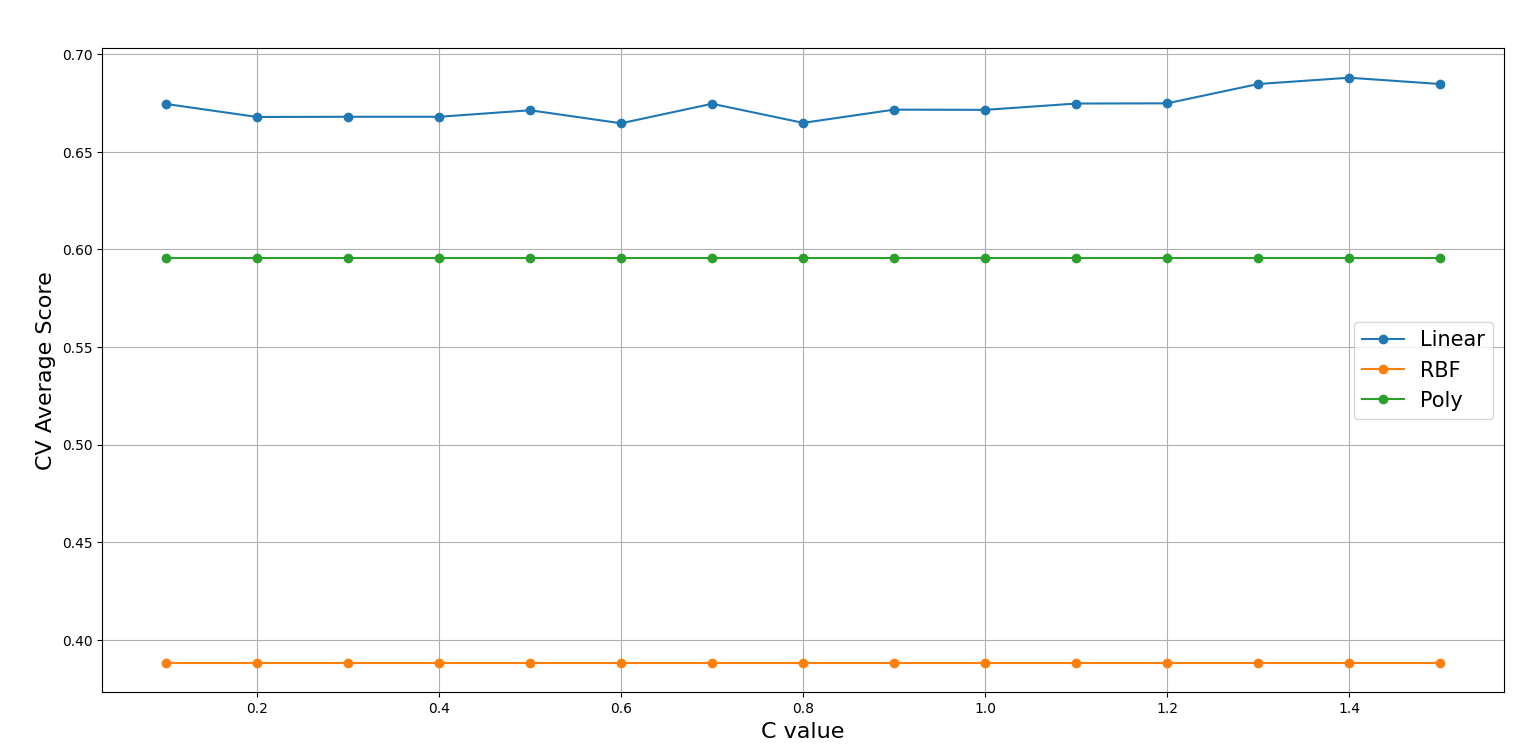
\includegraphics[scale=0.35]{svcCV.png}
		\caption{Grafico dell'andamento della media dell'accuratezza per ogni valore dell'iperparametro C e per ogni funzione kernel utilizzata durante l'applicazione della Cross Validation con 10 fold per il modello Support Vector Machine. Ogni punto è un classificatore con un certo valore di C. La linea blu indica l'andamento con la funzione linear kernel mentre la linea verde l'andamento con la funzione RBF e	la linea arancione l'andamento con la funzione polynomial kernel.
		} 
		\label{fig:svcCV}
	\end{center}
\end{figure}
Dal grafico si nota che, dal punto di vista dell'accuratezza registrata nel \emph{validation} \emph{set}, il kernel di tipo lineare ottiene le prestazioni migliori. Infatti, vediamo che la linea blu è costantemente al di sopra rispetto alle due restanti kernel a parità del valore in \textsf{C}. Invece, il polynomial kernel non ha buone prestazioni. Infatti, si registra che la linea arancione è costantemente al di sotto delle altre due linee, perché ha valori molto più bassi di accuratezza. Secondo la Cross Validation i risultati migliori sono stati il valore 1.4 per l'iperparametro \textsf{C} e il Linear kernel come funzione \textsf{kernel} da utilizzare. L'accuratezza ottenuta dal modello migliore nel \emph{validation} \emph{set} è stata di 0.789. Nella fase di predizione si sono ottenute le predizioni mostrate nella Figura \ref{fig:tabsvc} con le relative metriche presentate nella Figura \ref{fig:svcmetrics}.
\begin{figure}[]
	\begin{center}
		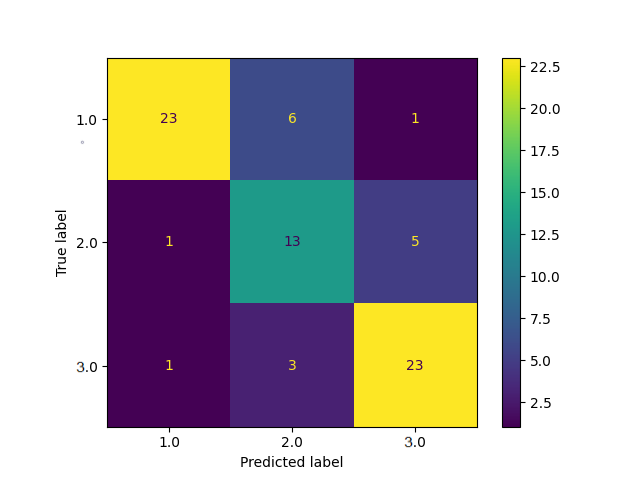
\includegraphics[scale=0.60]{tabsvc.png}
		\caption{Tabella di confusione del modello Support Vector Machine con \textsf{C} = 1.4 e \textsf{kernel} = linear. La classe 0.0 indica la vittoria della squadra in casa, la classe 1.0 indica il pareggio tra le due squadre, la classe 2.0 indica la vittoria della squadra ospite.
		} 
		\label{fig:tabsvc}
	\end{center}
\end{figure}
\begin{figure}[]
	\begin{center}
		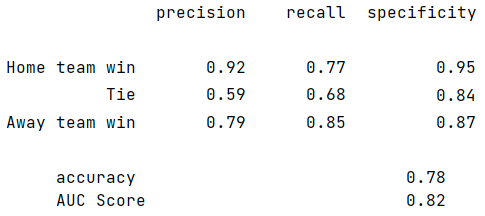
\includegraphics[scale=0.60]{metricsvc.png}
		\caption{Grafico delle misurazione durante la fase di predizione del modello Support Vector Machine con \textsf{C} = 1.4 e \textsf{kernel} = linear.
		} 
		\label{fig:svcmetrics}
	\end{center}
\end{figure}
Nonostante le poche osservazioni disponibili e l'elevato numero di \emph{features} utilizzate, i risultati ottenuti sono buoni. Infatti, l'accuratezza delle predizioni è pari a 0.78. Il modello riesce a riconoscere buona parte delle osservazioni di classe pareggio. Infatti, la sensibilità per la classe pareggio è pari a 0.68 ovvero, solo sei osservazioni di classe pareggio su 19 non sono state riconosciute come tali. Tuttavia, la precisione scende a 0.59. Infatti, nove osservazioni sono state etichettate erroneamente dal modello con la classe pareggio. Ciononostante, quest'errore non è molto grande dato che la specificità è pari a 0.84. Risultati migliori si ottengono per la classe vittoria della squadra in casa e vittoria della squadra ospite. La precisione per la classe della vittoria della squadra in casa è pari a 0.92. Infatti, solo due osservazioni sono state etichettate erroneamente dal modello con la classe vittoria della squadra in casa. Di conseguenza anche la specificità ha un valore molto alto ovvero pari a 0.95. Tuttavia, sette osservazioni di classe vittoria della squadra in casa non sono state identificate correttamente, infatti la sensibilità è pari a 0.77. Invece, la sensibilità della classe vittoria della squadra ospite è pari a 0.85 ovvero, solo quattro osservazioni non vengo identificate di classe vittoria della squadra ospite. Si rileva una precisione pari a 0.79 ovvero delle 29 osservazioni classificate con la classe vittoria della squadra ospite solo sei risultano essere di un'altra classe. Buone prestazioni anche per la specificità della classe vittoria della squadra ospite che è pari a 0.87.\\
L'algoritmo Support Vector Machine per quest'analisi si è rivelato particolarmente soddisfacente, nonostante la grande diversità da partita a partita e le poche osservazioni messe disposizione (380 partite).


\section{Decision Tree}

Con l'applicazione dell'algoritmo Decision Tree sono stati registrati dei buoni risultati durante la fase di predizione. Analogamente all'algoritmo K-Nearest-Neighbors, si è applicato la K-Fold Cross Validation con \emph{k = 10} per individuare i valori migliori per gli iperparametri.\\
Gli iperparametri valutati sono stati i seguenti:
\begin{itemize}
	\item \textsf{max\_depth}. Indica la profondità massima dell'albero di decisione. Si sono verificati valori che vanno da 3 fino a 52 con un aumento unitario di 1. Si sottolinea che 52 è il numero di \emph{feature} che sono presenti nel \emph{dataset}. Inoltre, questo parametro permette di controllare l'\emph{overfitting} ovvero, se le prestazioni peggiorano durante il training, i rami più profondi dell'albero vengono tagliati.
	\item \textsf{criterion}. Indica la regola di decisione utilizzata per la creazione dell'albero di decisione. Si sono verificate le regole Gini Index e Cross Entropy.
	\item \textsf{min\_samples\_split}. Indica il numero minimo di istanze richieste per dividere un nodo interno. Se la condizione non viene rispettata allora il nodo sarà una foglia attuando una potatura dell'albero di decisione.
\end{itemize}
Nella Figura \ref{fig:dtCV}  viene mostrato l'andamento della Cross Validation per ogni valore degli iperparametri.
\begin{figure}[h]
	\begin{center}
		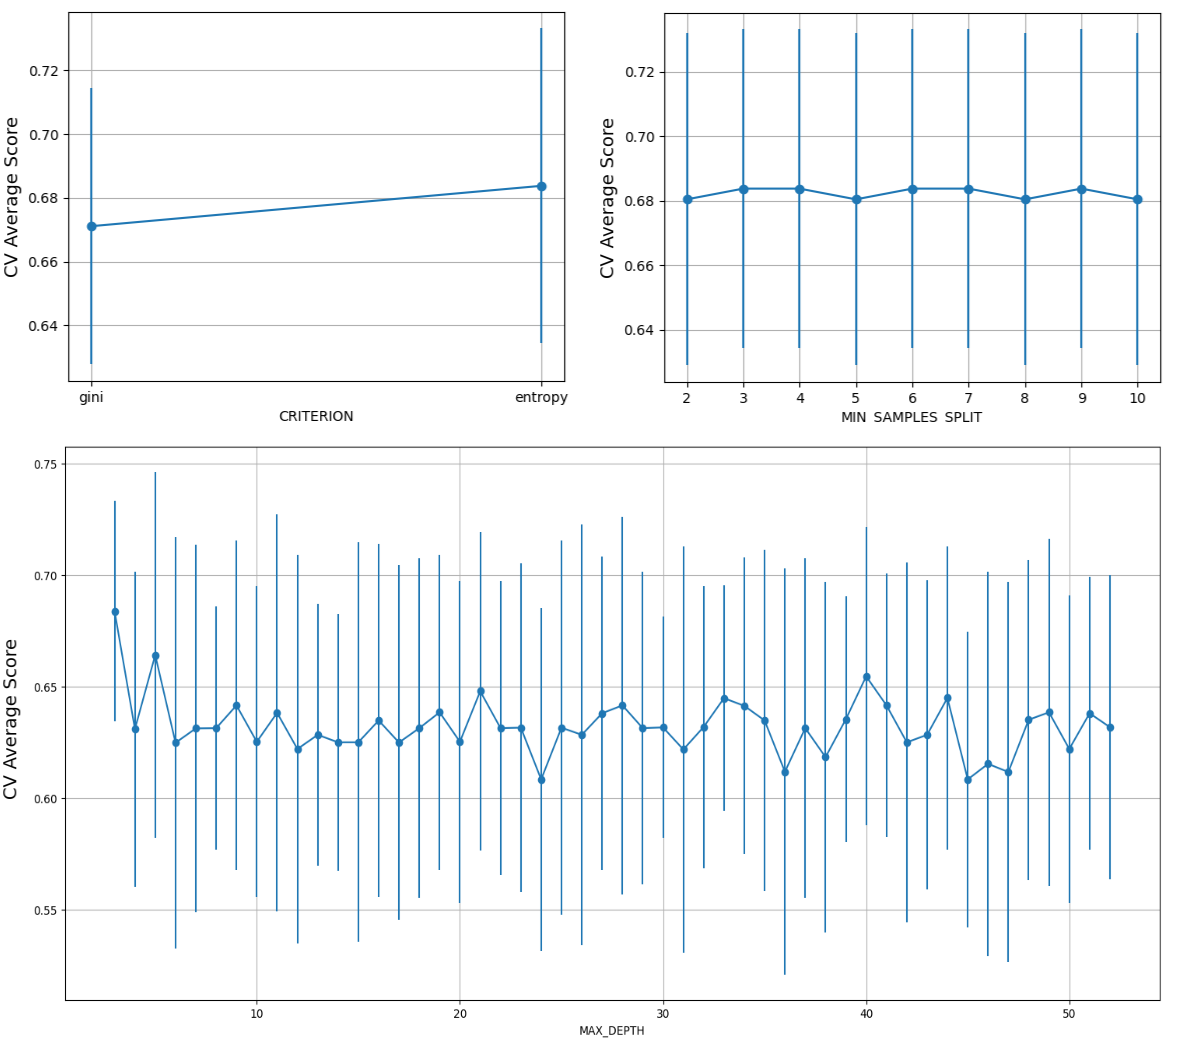
\includegraphics[scale=0.40]{dtCV.png}
		\caption{Il grafico in alto a sinistra indica l'andamento della media dell'accuratezza per ogni valore dell'iperparametro \textsf{criterion}. Il grafico in alto a destra indica l'andamento della media dell'accuratezza per ogni valore dell'iperparametro \textsf{min\_samples\_split}. Il grafico in basso indica l'andamento della media dell'accuratezza per ogni valore dell'iperparametro \textsf{max\_depth}. Entrambi i grafici sono l'applicazione della Cross Validation con 10 fold per il modello Decision Tree. 
		} 
		\label{fig:dtCV}
	\end{center}
\end{figure}
Dal grafico in alto a sinistra si nota che tra le due regole la migliore in termini di accuratezza media registrata nel \emph{validation set} è stata la Cross Entropy. Nel grafico in alto a destra i valori 3,4,6,7 e 9, assunti dall'iperparametro \textsf{min\_samples\_split} hanno fatto registrare le accuratezze medie più alte.\\
Nel grafico in basso vi è un andamento abbastanza irregolare. Si nota un forte decadimento delle prestazioni con l'aumento del valore del limite della profondità, soprattutto con valori superiore a 5. Secondo la Cross Validation i valori migliori sono stati il valore 3 sia per l'iperparametro \textsf{max\_depth} e sia per l'iperparametro \textsf{min\_samples\_split} e la Cross Entropy come regola di decisione da utilizzare. L'accuratezza ottenuta dal modello migliore nel \emph{validation} \emph{set} è stata di 0.684.\\
Nella fase di predizione si sono ottenute le predizioni mostrate nella Figura \ref{fig:tabdt} con le relative metriche presentate nella Figura \ref{fig:dtmetrics}.
\begin{figure}[h]
	\begin{center}
		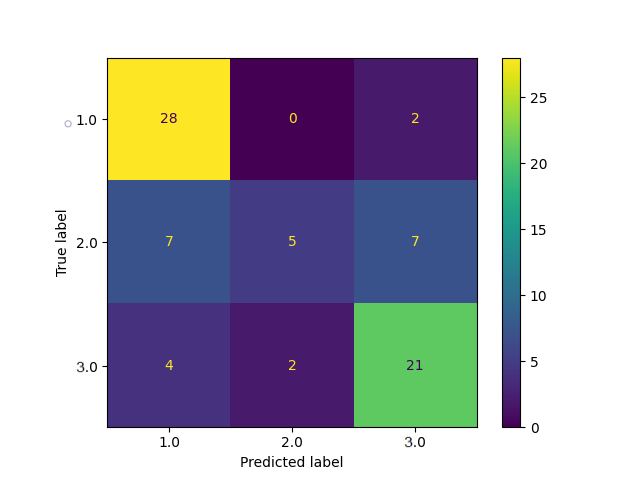
\includegraphics[scale=0.60]{tabdt.png}
		\caption{Tabella di confusione del modello Decision Tree con \textsf{max\_depth} = 3, \textsf{min\_samples\_split} = 3 e \textsf{criterion} = entropy. La classe 0.0 indica la vittoria della squadra in casa, la classe 1.0 indica il pareggio tra le due squadre, la classe 2.0 indica la vittoria della squadra ospite.
		} 
		\label{fig:tabdt}
	\end{center}
\end{figure}
\begin{figure}[]
	\begin{center}
		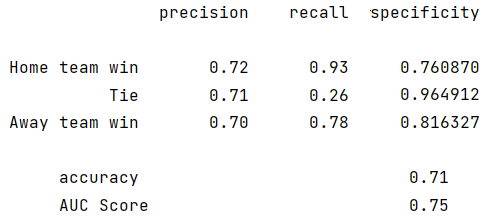
\includegraphics[scale=0.60]{metricdt.png}
		\caption{Grafico delle misurazione durante la fase di predizione del modello Decision Tree con \textsf{max\_depth} = 3, \textsf{min\_samples\_split} = 3 e \textsf{criterion} = entropy.
		} 
		\label{fig:dtmetrics}
	\end{center}
\end{figure}
Nonostante le poche osservazioni disponibili i risultati ottenuti sono buoni. Infatti, l'accuratezza delle predizioni è di 0.71. Il modello ha comunque qualche difficoltà a identificare le osservazioni della classe pareggio. Infatti, la sensibilità è pari a 0.26. Nonostante il modello etichetti un'osservazione con la classe pareggio in poche occasioni, esso sbaglia poco. Ci sono solo due osservazioni etichettate erroneamente con la classe pareggio, quindi la precisione è pari a 0.71. Ovviamente la specificità nella classe pareggio è molto alta dato che il modello poche volte sbaglia ad etichettare con la classe pareggio. Buoni risultati si ottengono sia per la classe vittoria della squadra in casa sia per la classe vittoria della squadra ospite. Infatti, per la prima classe c'è una sensibilità pari a 0.93, ovvero, soltanto due osservazioni di classe vittoria della squadra in casa non sono state identificate come tali. Le prestazioni però calano nella precisione dato che undici osservazioni sono state etichettate erroneamente con la classe vittoria della squadra in casa, registrando una precisione pari a 0.72. Di conseguenza anche la specificità è calata rispetto alla sensibilità con un valore pari a 0.76. La classe vittoria della squadra ospite ha una sensibilità pari a 0.78. Infatti, sei osservazioni di classe vittoria della squadra ospite non sono state identificate come tali. Anche la precisione rimane in linea con le prestazioni della sensibilità con un valore pari a 0.70, in cui nove osservazioni su trenta sono state etichettate erroneamente con la classe vittoria della squadra ospite. Nonostante ciò, la specificità è pari a 0.82.\\
Dato che l'algoritmo Decision Tree non è un algoritmo a scatola chiusa (\emph{black box}), è possibile capire quali sono state le sue scelte analizzando l'albero di decisione che ha prodotto per svolgere le sue predizioni. Nella Figura \ref{fig:dttree} viene mostrato l'albero di decisione prodotto e utilizzato durante la fase di predizione.
\begin{figure}[h]
	\begin{center}
		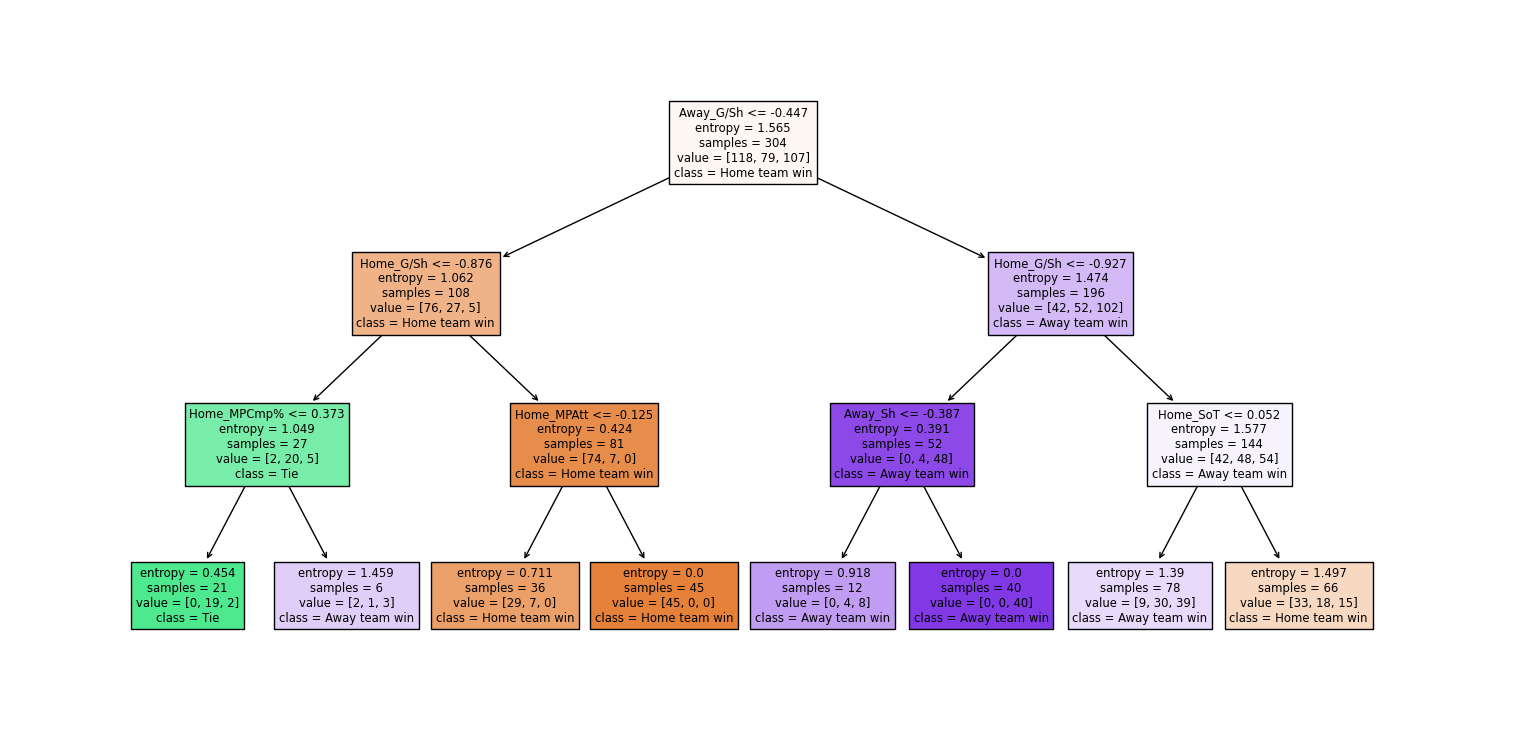
\includegraphics[height = 10cm, width = 16cm]{treedt.png}
		\caption{L'albero di decisione del modello Decision Tree con \textsf{max\_dept}h = 3 e \textsf{criterion} = entropy. Per ogni nodo non foglia c'è un test che indica quale ramo scegliere asseconda del valore contenuto nell'attributo testato. Il parametro \textsf{entropy} indica l'entropia misurata. Il parametro \textsf{samples} indica il numero di istanze che soddisfano i test precedenti. Nel parametro \textsf{value} vengono riportati il numero di istanze presenti per ognuna delle tre classi. Il parametro \textsf{class} indica la classe di maggioranza nel nodo. Il colore indica la classe di maggioranza con una tonalità differente asseconda della frequenza della classe di maggioranza.
		} 
		\label{fig:dttree}
	\end{center}
\end{figure}
Nell'albero mostrato in Figura \ref{fig:dttree}, per ogni nodo non foglia c'è un test che indica quale ramo scegliere a seconda del valore contenuto nell'attributo testato. Il test consiste semplicemente nel verificare se l'attributo ha un valore minore o uguale oppure maggiore rispetto a una certa soglia. Questo tipo di test permette di gestire attributi con valori continui utilizzando una soglia di decisione scelta opportunamente dell'algoritmo. Per tutti i nodi è presente il parametro \textsf{entropy} che indica l'entropia misurata. Il parametro \textsf{samples} che indica il numero di istanze che soddisfano i test precedenti. Il parametro \textsf{value} che il numero di istanze presenti per ognuna delle tre classi. Il parametro \textsf{class} che indica la classe di maggioranza nel nodo, mentre il colore indica la classe di maggioranza con una tonalità differente a seconda della frequenza della classe di maggioranza. Quando viene raggiunto un nodo foglia si classifica l'osservazione con la classe di maggioranza dato che non ci sono più attributi che permettono di distinguere le istanze.\\
Osservando l'albero, le \emph{feature} legate ai tiri si confermano di grande importanza non solo i modelli Bradley-Terry visti nel Capitolo \ref{cap:risultatiDM}, ma anche per il modello Decision Tree.\\
In conclusione, l'algoritmo Decision Tree ottiene delle buone prestazioni pur rimanendo semplice senza diventare troppo complesso.

\section{Random Forest}
Con l'applicazione dell'algoritmo Random Forest si sono registrati dei buoni risultati durante la fase di predizione. Analogamente all'algoritmo K-Nearest-Neighbors, si è applicato la K-Fold Cross Validation con \emph{k = 10} per individuare i valori migliori per gli iperparametri.\\
Gli iperparametri valutati sono stati i seguenti:
\begin{itemize}
	\item \textsf{criterion}. Indica la regola di decisione utilizzata per la creazione degli alberi di decisione. Si sono verificate le regole Gini Index e Cross Entropy.
	\item \textsf{max\_depth}. Indica la profondità massima degli alberi di decisione utilizzati. Si sono verificati valori che vanno da 3 fino a 52 con un aumento unitario di 1. Si sottolinea che 52 è il numero di \emph{feature} che sono presenti nel \emph{dataset}. Inoltre, questo parametro permette di controllare l'\emph{overfitting} ovvero, se le prestazioni peggiorano durante il training, i rami più profondi dell'albero vengono tagliati.
	\item \textsf{n\_estimators}. Indica il numero massimo di classificatori impiegati per il Bagging. Si sono verificati valori che vanno da 3 fino a 126 classificatori con un aumento unitario di 1.
	\item \textsf{min\_samples\_split}. Indica il numero minimo di istanze richieste per dividere un nodo interno. Se la condizione non viene rispettata allora il nodo sarà una foglia attuando una potatura dell'albero di decisione.
\end{itemize}
Nella Figura \ref{fig:rfCV} viene mostrato l'andamento della Cross Validation per ogni valore degli iperparametri.
\begin{figure}[]
	\begin{center}
		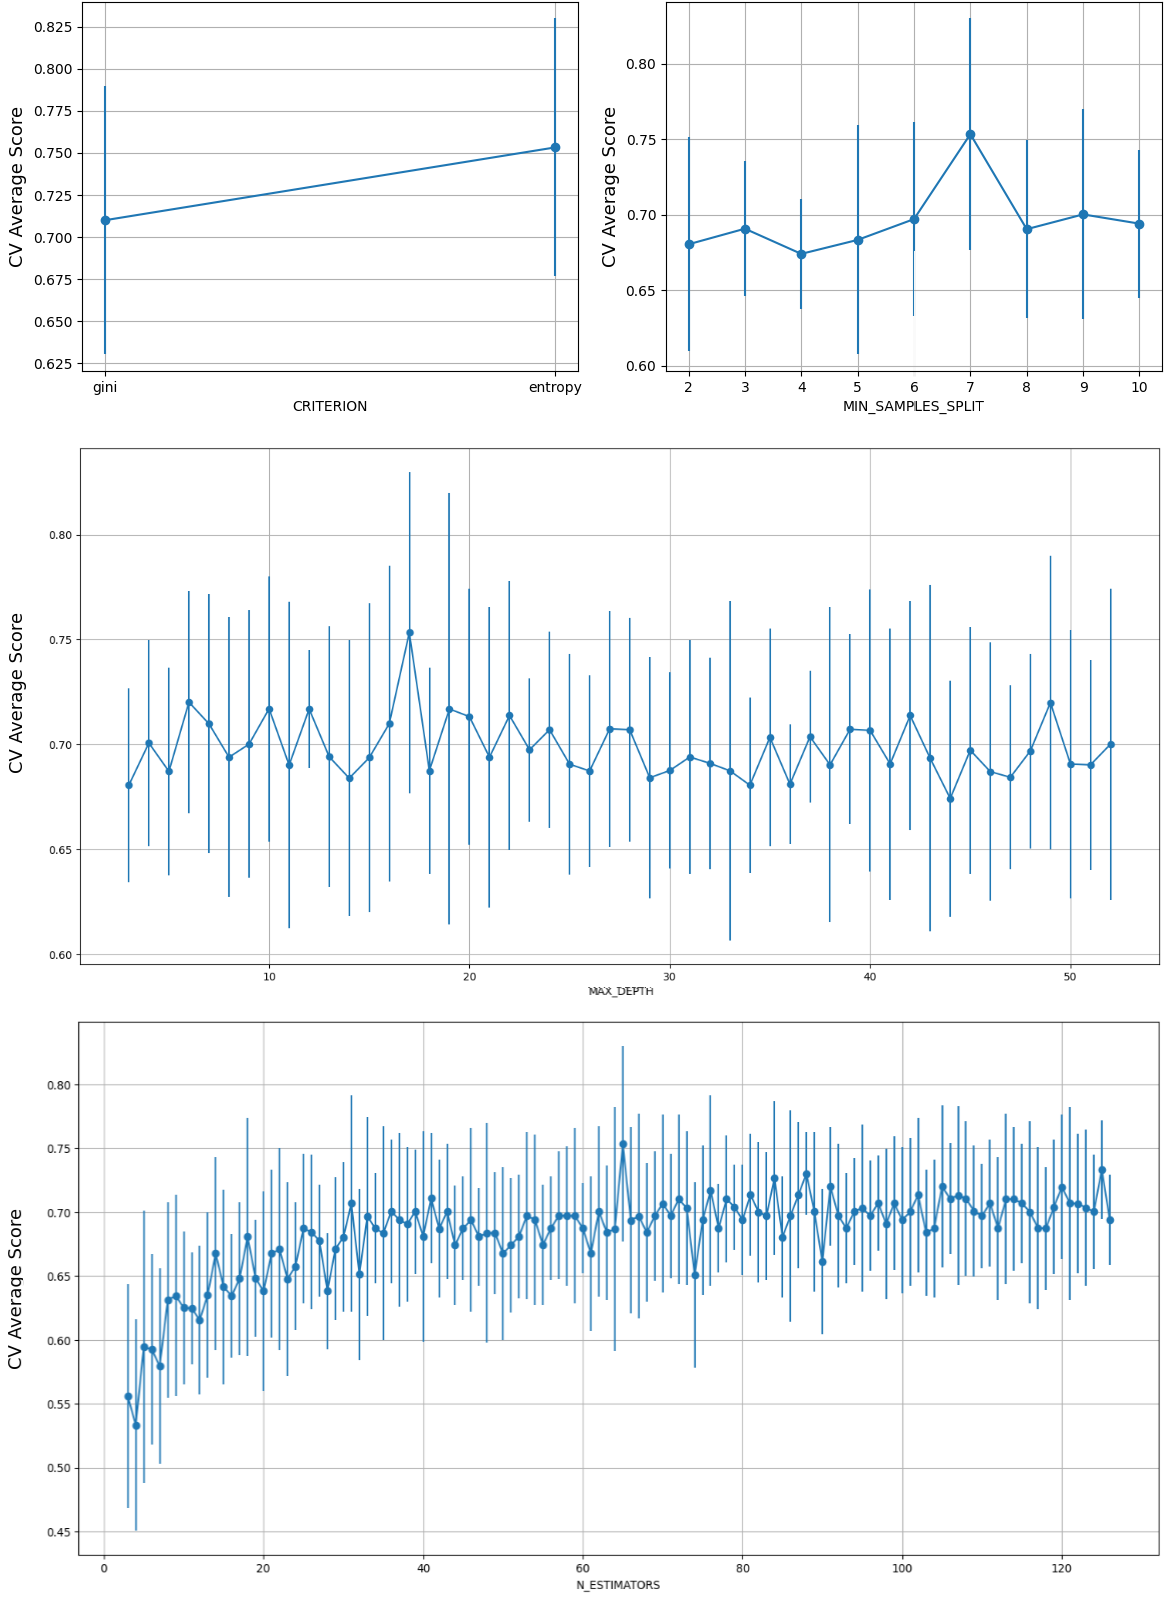
\includegraphics[scale=0.40]{rfCV.png}
		\caption{Il grafico in alto a sinistra indica l'andamento della media dell'accuratezza per ogni valore dell'iperparametro \textsf{criterion}. Il grafico in alto a destra indica l'andamento della media dell'accuratezza per ogni valore dell'iperparametro \textsf{min\_samples\_split}. Il grafico al centro indica l'andamento della media dell'accuratezza per ogni valore dell'iperparametro \textsf{max\_depth}. Il grafico in basso indica l'andamento della media dell'accuratezza per ogni valore dell'iperparametro \textsf{n\_estimators}. Tutti i grafici sono l'applicazione della Cross Validation con 10 fold per il modello Random Forest. 
		} 
		\label{fig:rfCV}
	\end{center}
\end{figure}
Dal grafico in alto a sinistra si nota che tra le due regole la migliore in termini di accuratezza media registrata nel \emph{validation set} è stata la Cross Entropy. Nel grafico in alto a destra con il valore 7 nell'iperparametro \textsf{min\_samples\_split} il modello ottiene l'accuratezza media più alta. Nel grafico al centro vi è un andamento abbastanza irregolare. Si nota che con il valore 17 dell'iperparametro \textsf{max\_depth} vi è un aumento improvviso del valore dell'accuratezza media del modello. Infine, anche nel grafico in basso vi è un andamento abbastanza irregolare. Nonostante un'iniziale tendenza di aumento dell'accuratezza. Quando l'iperparametro \textsf{n\_estimators} assume il valore 65 vi è un picco di prestazione dell'accuratezza media.\\
Secondo la Cross Validation i valori migliori sono stati per l'iperparametro \textsf{criterion} la Cross Entropy, il valore 17 per l'iperparametro \textsf{max\_depth}, per l'iperparametro \textsf{min\_samples\_split} il valore 7 e per l'iperparametro \textsf{n\_estimators} il valore 65 come numero di classificatori da impiegare.
L'accuratezza ottenuta dal modello migliore nel \emph{validation} \emph{set} è stata di 0.753.\\
Nella fase di predizione si sono ottenute le predizioni mostrate nella Figura \ref{fig:tabrf} con le relative metriche presentate nella Figura \ref{fig:rfmetrics}.
\begin{figure}[h]
	\begin{center}
		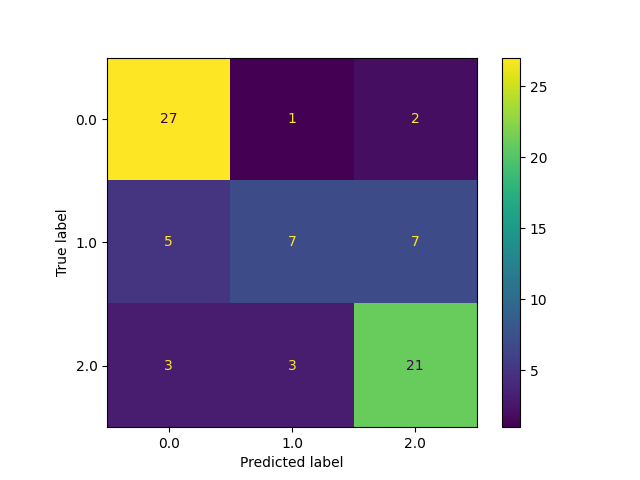
\includegraphics[scale=0.60]{tabrf.png}
		\caption{Tabella di confusione del modello Random Forest con \textsf{criterion} = gini, \textsf{max\_depth} = 5, \textsf{n\_estimators} = 102 e \textsf{min\_samples\_split} = 9. La classe 0.0 indica la vittoria della squadra in casa, la classe 1.0 indica il pareggio tra le due squadre, la classe 2.0 indica la vittoria della squadra ospite.
		} 
		\label{fig:tabrf}
	\end{center}
\end{figure}

\begin{figure}[]
	\begin{center}
		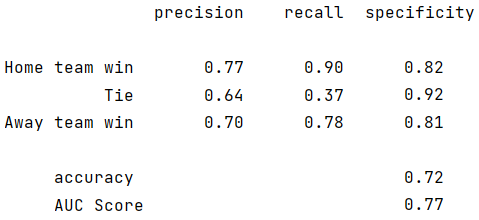
\includegraphics[scale=0.60]{metricrf.png}
		\caption{Grafico delle misurazione durante la fase di predizione del modello Random Forest con \textsf{criterion} = gini, \textsf{max\_depth} = 5, \textsf{n\_estimators} = 102 e \textsf{min\_samples\_split} = 9.
		} 
		\label{fig:rfmetrics}
	\end{center}
\end{figure}
Nonostante le poche osservazioni disponibili i risultati ottenuti sono buoni. Infatti, l'accuratezza delle predizioni e di 0.72. Anche in questo modello si sono riscontrate alcune difficoltà nell'identificare le istanze della classe pareggio. La sensibilità rilevata sulla classe pareggio è pari a 0.37, perché solo sette osservazioni su 19 osservazioni di classe pareggio sono state identificate con la classe pareggio. Tuttavia, le prestazioni migliorano con la precisione del modello nell'etichettare un'istanza con la classe pareggio, infatti delle undici osservazioni classificate con la classe pareggio solo quattro sono risultate essere di una classe differente. Di conseguenza anche la specificità sulla classe pareggio ha un valore alto pari a 0.92. Si registrano prestazioni migliori con le classi vittoria della squadra in casa e vittoria della squadra ospite. Per la classe vittoria della squadra in casa si ha una sensibilità pari a 0.90 ovvero, solo tre osservazioni su 30 non sono state riconosciute di classe vittoria della squadra in casa. Tuttavia, si registra un calo di prestazioni nella precisione nell'etichettare correttamente le istanze di classe vittoria della squadra in casa. Infatti, si registra un valore pari a 0.77 perché otto osservazioni sono state classificate erroneamente con la classe vittoria della squadra in casa. Di conseguenza anche la specificità sulla classe della vittoria della squadra in casa cala, raggiungendo un valore pari a 0.82. Buone prestazioni del modello si rilevano nell'identificare le istanze di classe vittoria della squadra ospite, con una sensibilità pari a 0.78. Purtroppo, si registra una precisione più bassa ovvero pari a 0.70, con nove osservazioni classificate erroneamente con la classe vittoria della squadra ospite. Infine, la specificità del modello sulla classe vittoria della squadra ospite è pari a 0.81.\\
Dato che l'algoritmo Random Forest utilizza i classificatori Decision Tree è possibile capire quali sono le \emph{features} più importanti secondo il modello per produrre una predizione dell'esito di una partita. Perciò, nella Figura \ref{fig:rftree} viene mostrato per ogni \emph{feature} la sua importanza misurata sull'impurità.
\begin{figure}[]
	\begin{center}
		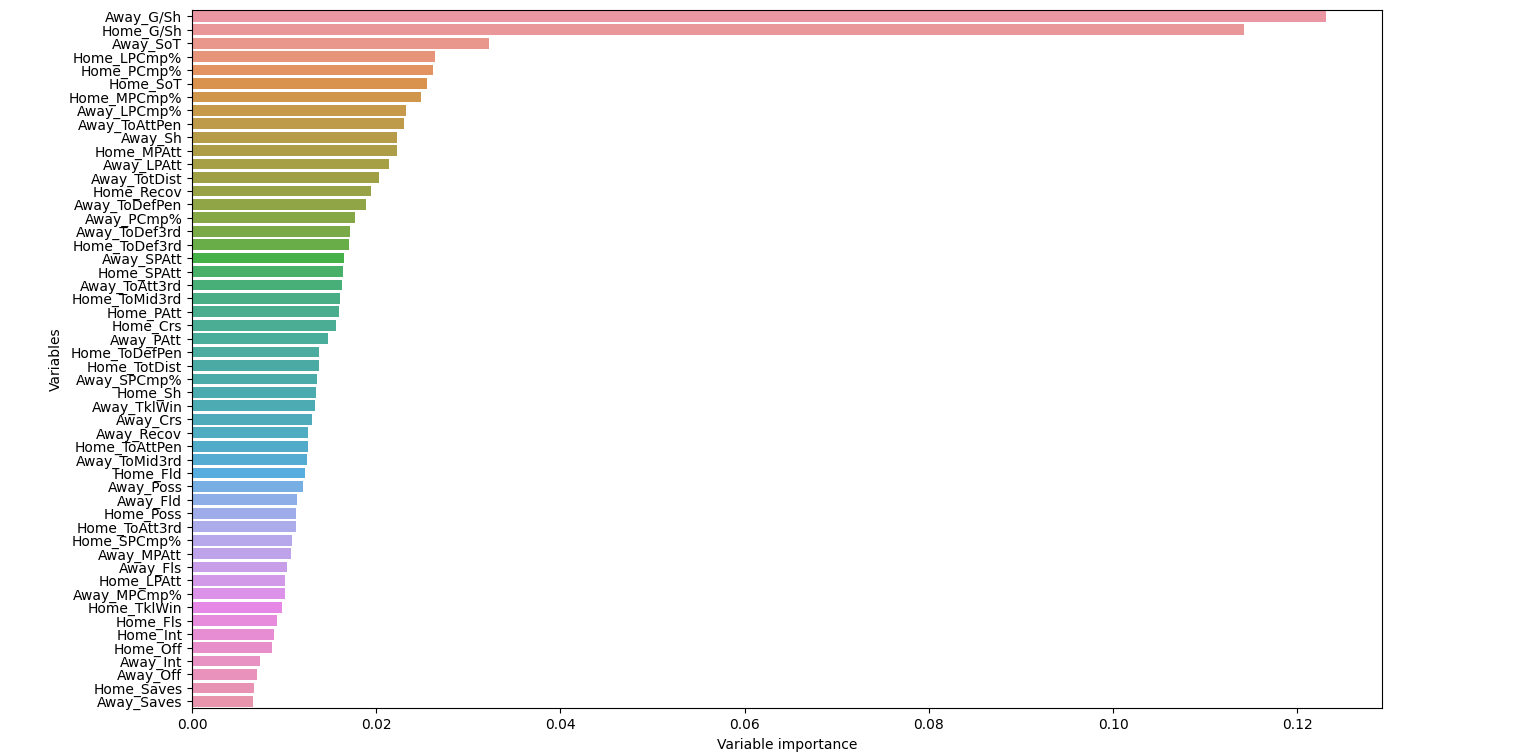
\includegraphics[height = 10cm, width = 14cm]{rfCV5.png}
		\caption{Il grafico riporta per ogni \emph{feature} la sua importanza basata sull'impurità.
		} 
		\label{fig:rftree}
	\end{center}
\end{figure}
Osservando i risultati ottenuti essi sono coerenti con quanto visto nell'albero del Decision tree e con i risultati ottenuti dai modelli Bradley-Terry illustrati nel Capitolo \ref{cap:risultatiDM}. Le \emph{features} legate ai tiri si confermano di grande importanza, così come i passaggi completati, soprattutto i passaggi lunghi. Tuttavia, si nota una differenza di importanza tra i modelli Bradley-Terry e il Random Forest: il numero di parate fatte è significativo per i modelli Bradley-Terry, mentre per il Random Forest è la feature meno importante.\\
In conclusione, nonostante le poche osservazioni disponibili, l'algoritmo Random Forest ottiene nel complesso delle buone prestazioni, nonostante qualche difficoltà nell’identificazione dei pareggi.

\section{AdaBoost}
Con l'applicazione dell'algoritmo AdaBoost si sono registrati dei buoni risultati durante la fase di predizione. Analogamente all'algoritmo K-Nearest-Neighbors, si è applicato la K-Fold Cross Validation con \emph{k = 10} per individuare i valori migliori per gli iperparametri.\\
Gli iperparametri valutati sono stati i seguenti:
\begin{itemize}
	\item \textsf{n\_estimators}. Indica il numero massimo di classificatori impiegati per il Boosting. Si sono verificati valori che vanno da 3 fino a 126 classificatori con un aumento unitario di 1.
	\item \textsf{learning\_rate}. Indica il peso applicato ad ogni classificatore per ogni iterazione del Boosting. Si sono verificati valori che vanno da 0.1 fino a 1.0 con un aumento unitario di 0.1. Più l'\textsf{learning\_rate} è elevato più sarà il contributo di ciascun classificatore.
\end{itemize}
Esiste un \emph{trade-off} tra i parametri \textsf{learning\_rate} e \textsf{n\_estimators}. Nella Figura \ref{fig:adaCV} viene mostrato l'andamento della Cross Validation per ogni valore degli iperparametri.
\begin{figure}[h]
	\begin{center}
		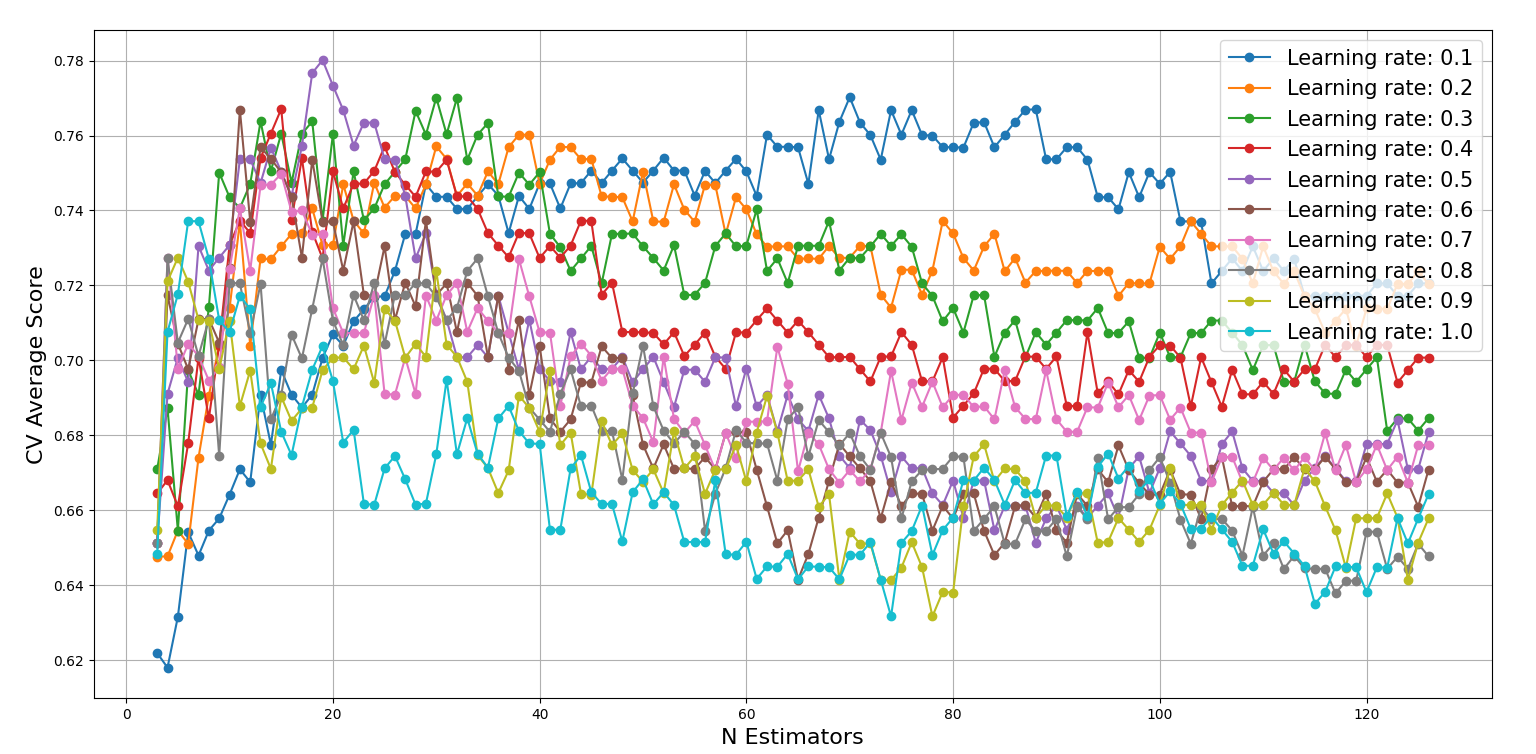
\includegraphics[scale=0.35]{adaCV.png}
		\caption{Grafico dell'andamento della media dell'accuratezza per ogni valore dell'iperparametro \textsf{n\_estimators} e per ogni valore dell'iperparametro \textsf{learning\_rate} utilizzati durante l'applicazione della Cross Validation con 10 fold per il modello AdaBoost. Ogni punto utilizza un certo numero classificatori mentre il colore indica il peso dell'\emph{learning rate}.
		} 
		\label{fig:adaCV}
	\end{center}
\end{figure}
Dal grafico, notiamo un andamento abbastanza irregolare per quasi tutti i tassi d'apprendimento, eccetto per il modello con il tasso d'apprendimento pari a 0.1, il quale inizialmente ottiene prestazioni migliori con il salire del numero dei classificatori. Tutti i tassi d'apprendimento con un numero elevato di classificatori calano il loro valore di accuratezza nel \emph{validation set}. Nonostante il modello con \textsf{learning\_rate} pari a 0.1 abbia costantemente valori più alti, il modello con \textsf{learning\_rate} pari a 0.5 ha segnato un'accuratezza più alta anche se, con l'aumentare del numero di classificatori, le sue prestazioni calano di molto. \\
Perciò, secondo la Cross Validation i valori migliori sono stati il valore 19 per l'iperparametro \textsf{n\_estimators} e il valore 0.5 per l'iperparametro \textsf{learning\_rate}. L'accuratezza ottenuta dal modello migliore nel \emph{validation} \emph{set} è stata di 0.78.\\
Nella fase di predizione si sono ottenute le predizioni mostrate nella Figura \ref{fig:tabada} con le relative metriche presentate nella Figura \ref{fig:adametrics}.
\begin{figure}[h]
	\begin{center}
		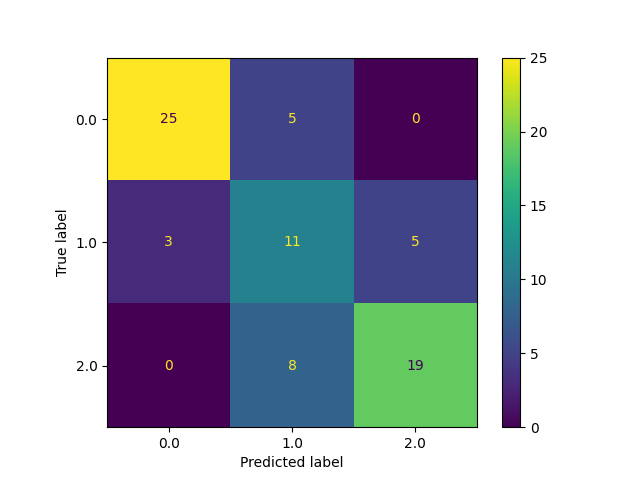
\includegraphics[scale=0.60]{tabada.png}
		\caption{Tabella di confusione del modello AdaBoost con \textsf{n\_estimators} = 19 e \textsf{learning\_rate} = 0.5. La classe 0.0 indica la vittoria della squadra in casa, la classe 1.0 indica il pareggio tra le due squadre, la classe 2.0 indica la vittoria della squadra ospite.
		} 
		\label{fig:tabada}
	\end{center}
\end{figure}

\begin{figure}[h]
	\begin{center}
		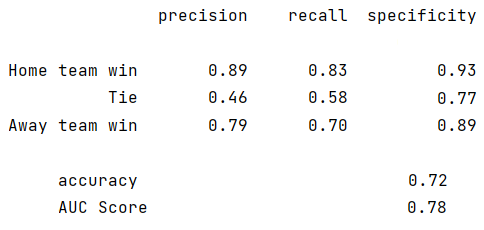
\includegraphics[scale=0.60]{metricada.png}
		\caption{Grafico delle misurazione durante la fase di predizione del modello AdaBoost con \textsf{n\_estimators} = 19 e \textsf{learning\_rate} = 0.5.
		} 
		\label{fig:adametrics}
	\end{center}
\end{figure}
Nonostante le poche osservazioni disponibili i risultati ottenuti sono buoni. Infatti, l'accuratezza delle predizioni è di 0.72. Anche questo modello ha delle difficoltà a identificare le istanze di classe pareggio. La sensibilità del modello sulla classe pareggio è pari a 0.58 ovvero, undici osservazioni su 19 di classe pareggio sono state identificate come tali. Purtroppo, il modello non è abbastanza soddisfacente nell’etichettare le istanze con la classe pareggio perché la precisione è pari a 0.46. Di conseguenza anche la specificità ne risente, con un valore pari a 0.77. Tuttavia, le prestazioni sono decisamente migliori con le classi vittoria della squadra in casa e vittoria della squadra ospite. Infatti, per la classe vittoria della squadra in casa la sensibilità è pari a 0.83, cioè solo cinque osservazioni su 30 non sono state riconosciute di classe vittoria della squadra. Analogamente, la specificità della classe vittoria della squadra in casa ha un valore molto alto ovvero, 0.93. Inoltre, il modello risulta essere molto preciso nel classificare correttamente le istanze con la classe vittoria della squadra in casa. Infatti, il modello ha commesso solo tre errori ottenendo una precisione pari a 0.89. Buone prestazioni si sono registrate anche nell'identificare le istanze di classe vittoria della squadra ospite da parte del modello. La sensibilità è pari a 0.70, mentre la precisione è pari a 0.79, con solo cinque osservazioni classificate erroneamente con la classe vittoria della squadra ospite. Buona anche la specificità del modello sulla classe vittoria della squadra ospite che risulta essere pari a 0.89.\\
In conclusione, nonostante le poche osservazioni messe a disposizione, l'algoritmo AdaBoost ottiene nel complesso delle buone prestazioni nonostante qualche difficoltà nell’identificazione dei pareggi.

\section{Comparazione dei algoritmi}
Grazie alla metrica AUC è possibile confrontare le performance degli algoritmi utilizzati. 
Nella Figura \ref{fig:auc} vengono riportate le AUC che sono state misurate durante la fase di predizione di ogni algoritmo utilizzato.

\begin{figure}[h]
	\begin{center}
		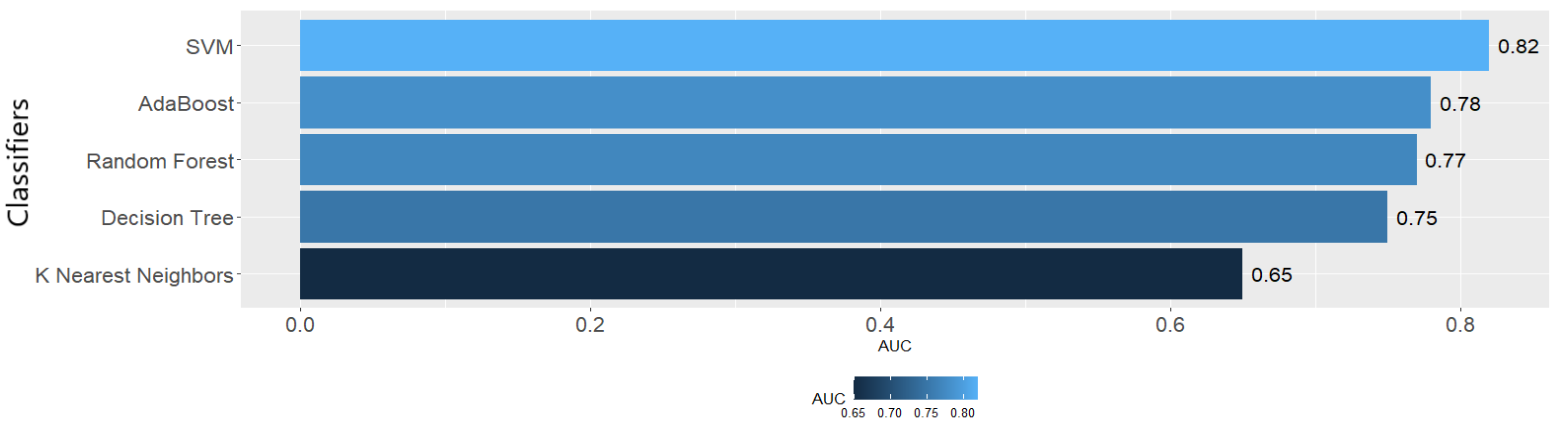
\includegraphics[scale=0.30]{auc.png}
		\caption{Grafico a barre in cui viene riportata la Area Under the Curve (AUC) registrata durante la fase di predizione dei algoritmi K-Nearest-Neighbors (K-NN),  Support Vector Machine (SVM), Decision Tree, Random Forest e AdaBoost.  
		} 
		\label{fig:auc}
	\end{center}
\end{figure}
Dalle misurazioni ottenute si evince che l'AUC più alta è stata registrata nell'algoritmo SVM con un valore pari a 0.82. Infatti, la SVM ha una buona accuratezza perché è l'algoritmo che riesce a identificare con maggior precisione la classe pareggio, la quale è risultata molto ostica da identificare per gli algoritmi trattati. Con una AUC leggermente inferiore, l'algoritmo AdaBoost si classifica come secondo con un valore pari a 0.78. Analogamente alla SVM, l'AdaBoost si distingue dai algoritmi con prestazioni inferiori grazie alle discrete prestazioni nell'identificazione della classe pareggio. L'algoritmo con la terza AUC più alta è stato il Random Forest con una AUC pari a 0.77 e con prestazioni simili all'algoritmo AdaBoost.
In quarta posizione si piazza l'algoritmo Decision Tree con una AUC pari a 0.75. Nonostante le buone prestazioni registrate nell'identificazione delle classi vittoria della squadra in casa e vittoria della squadra ospite, l'algoritmo Decision Tree paga una minor AUC a causa delle brutte prestazioni registrate nell'identificazione della classe pareggio. Infine, l'algoritmo con la più bassa AUC misurata è il K-NN con una AUC pari a 0.65. Infatti, l'algoritmo K-NN ha registrato delle pessime prestazioni nell'identificare le istanze di classe pareggio e delle discrete prestazioni nell'identificare le istanze delle altre due classi.\\
In conclusione, il problema presentato risulta essere troppo complesso per l'algoritmo K-NN: la strategia di classificare una nuova istanza con la classe di maggioranza dei k-vicini, seppur semplice, non è risultata efficace. Viceversa, la SVM, grazie all'utilizzo della funzione kernel, riesce a gestire la complessità dei dati ottenendo delle buone prestazioni in fase di predizione.
